\section{Drift Chambers (DC)}

\subsection{Geometry}

The FTOF geometry is implemented through the COATJAVA geometry service.
The service provides the geant4 definitions that are read by the GEMC perl api to build the geometry database.

Each layer is a generic G4Trapezoid, tilted by $+6^O$ or $-6^O$ depending if they are part of a stereo superlayer or not.
The 12 layers in each region (6 per superlayer) are placed in a region mother volume made of air, see \F{dcGeometry}.

\begin{figure}
	\centering
	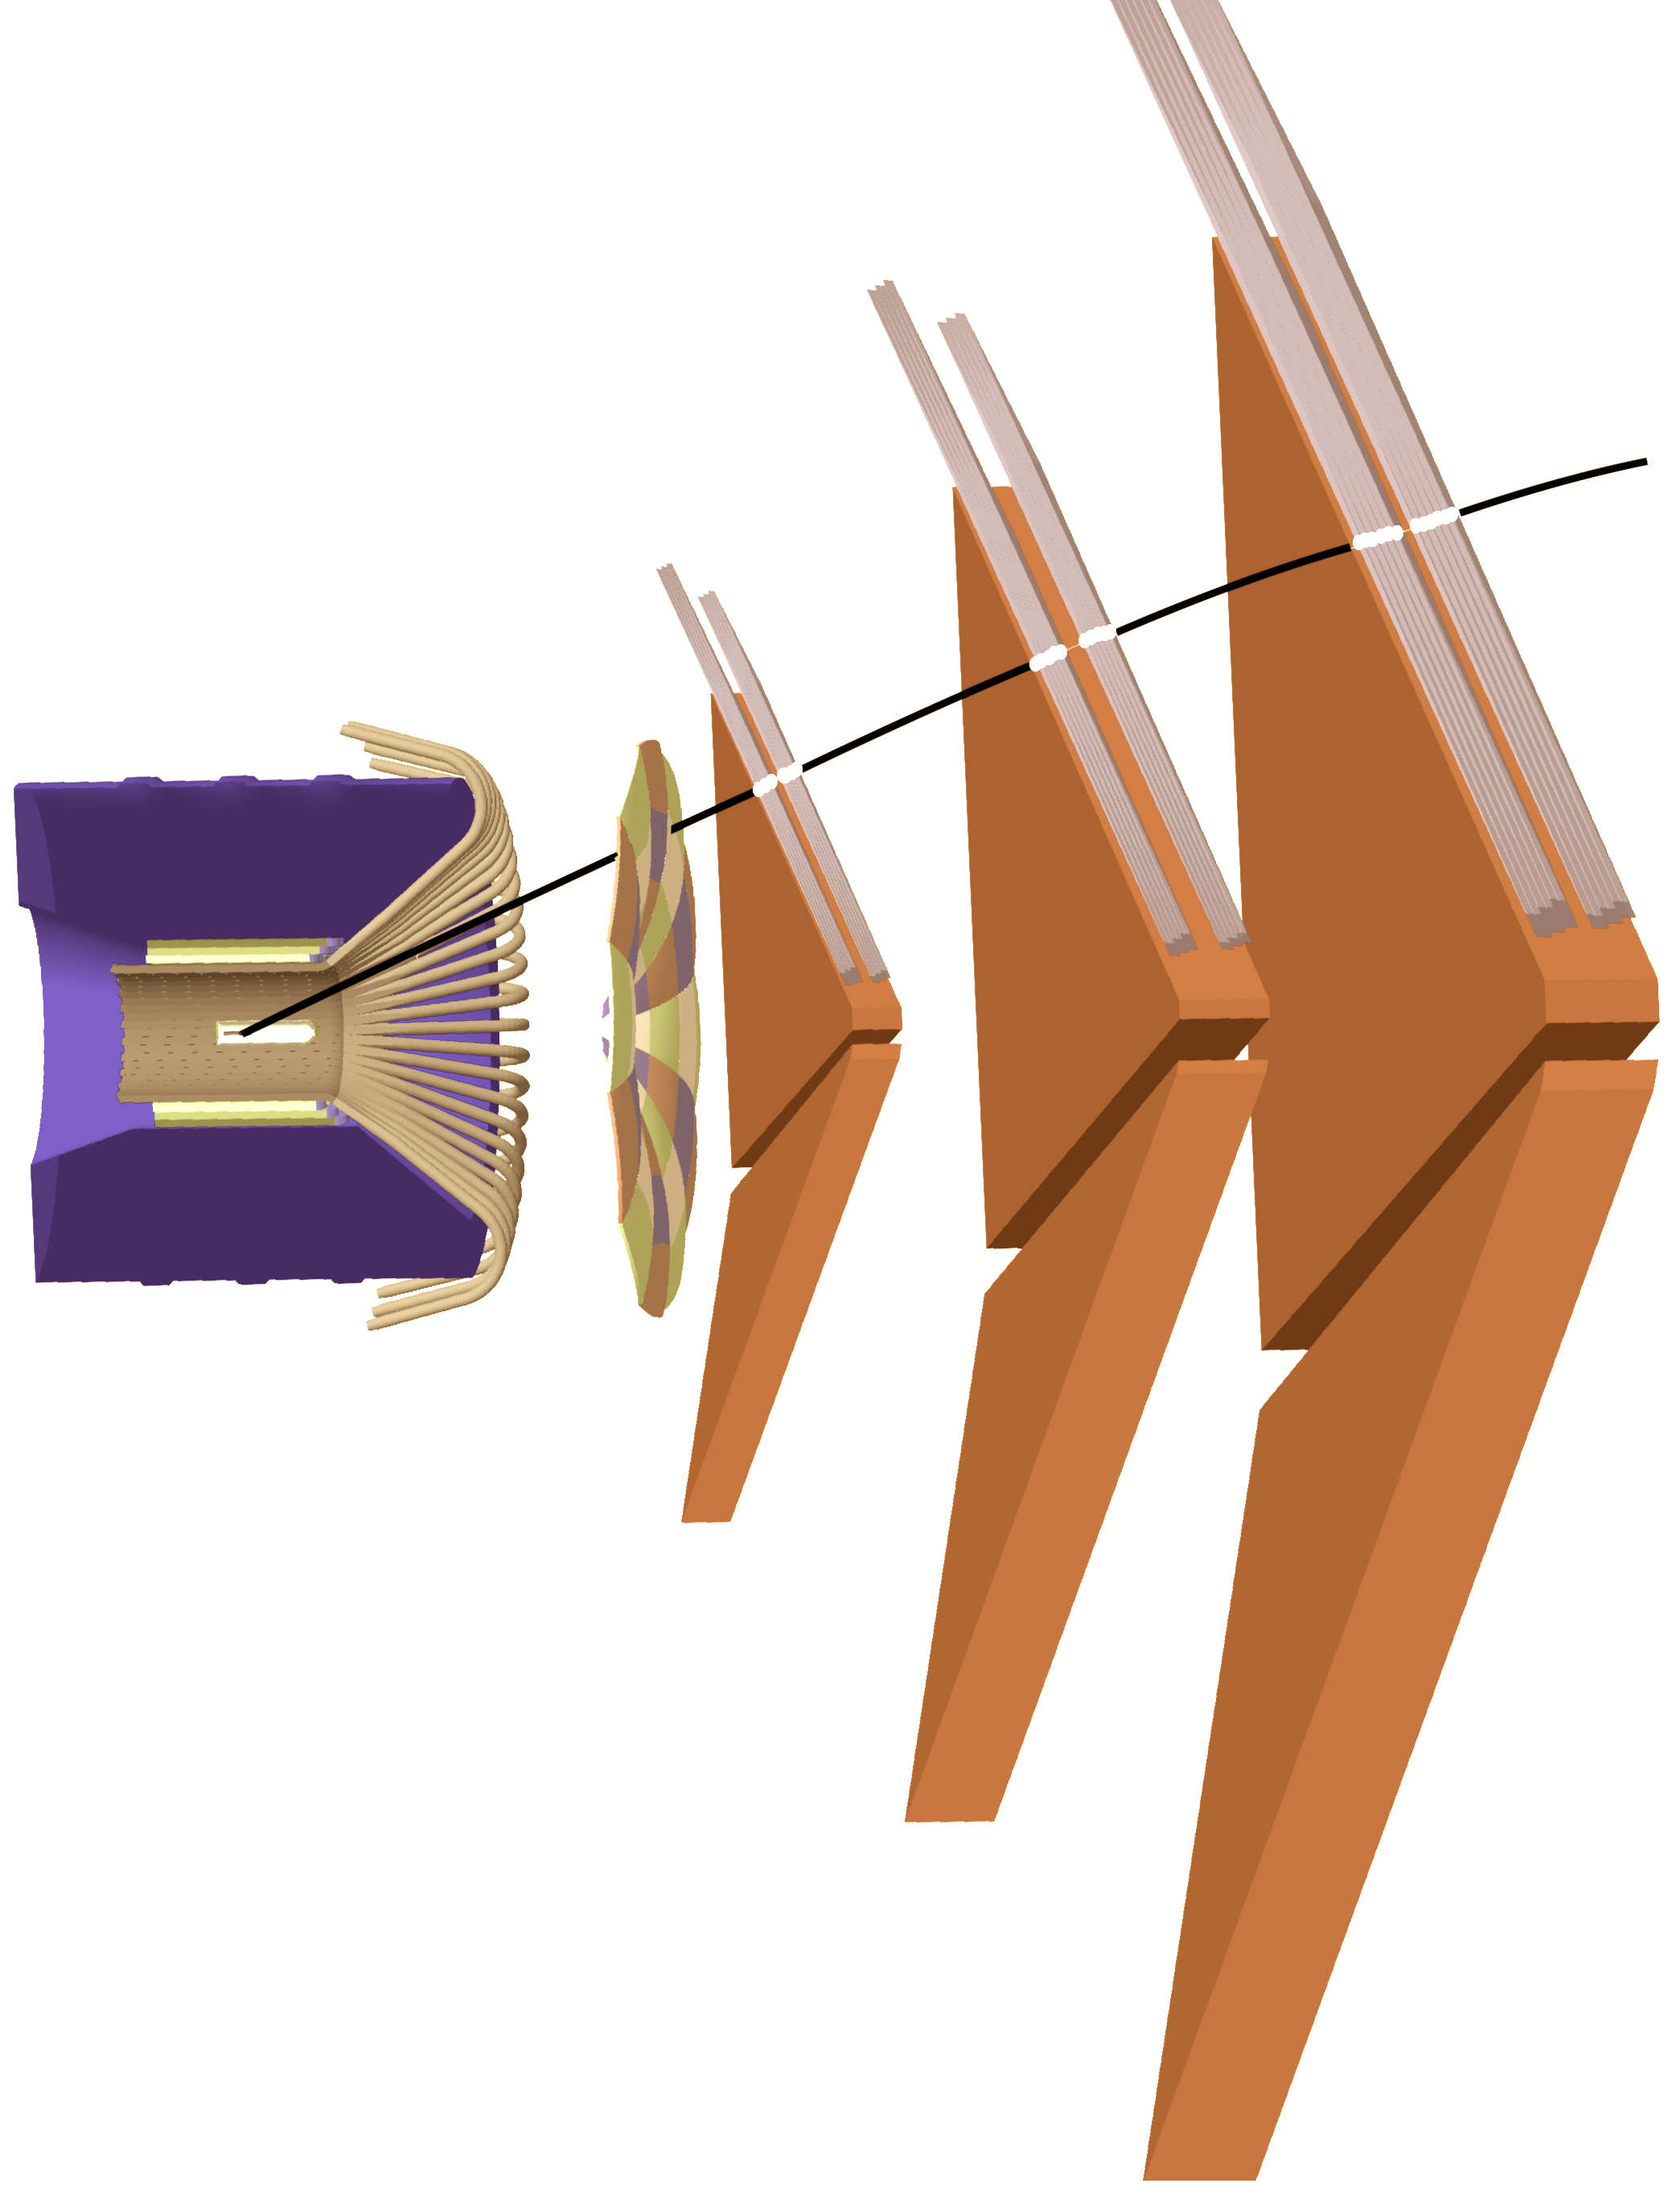
\includegraphics[width=0.95\columnwidth,keepaspectratio]{img/dcGeometry.png}
	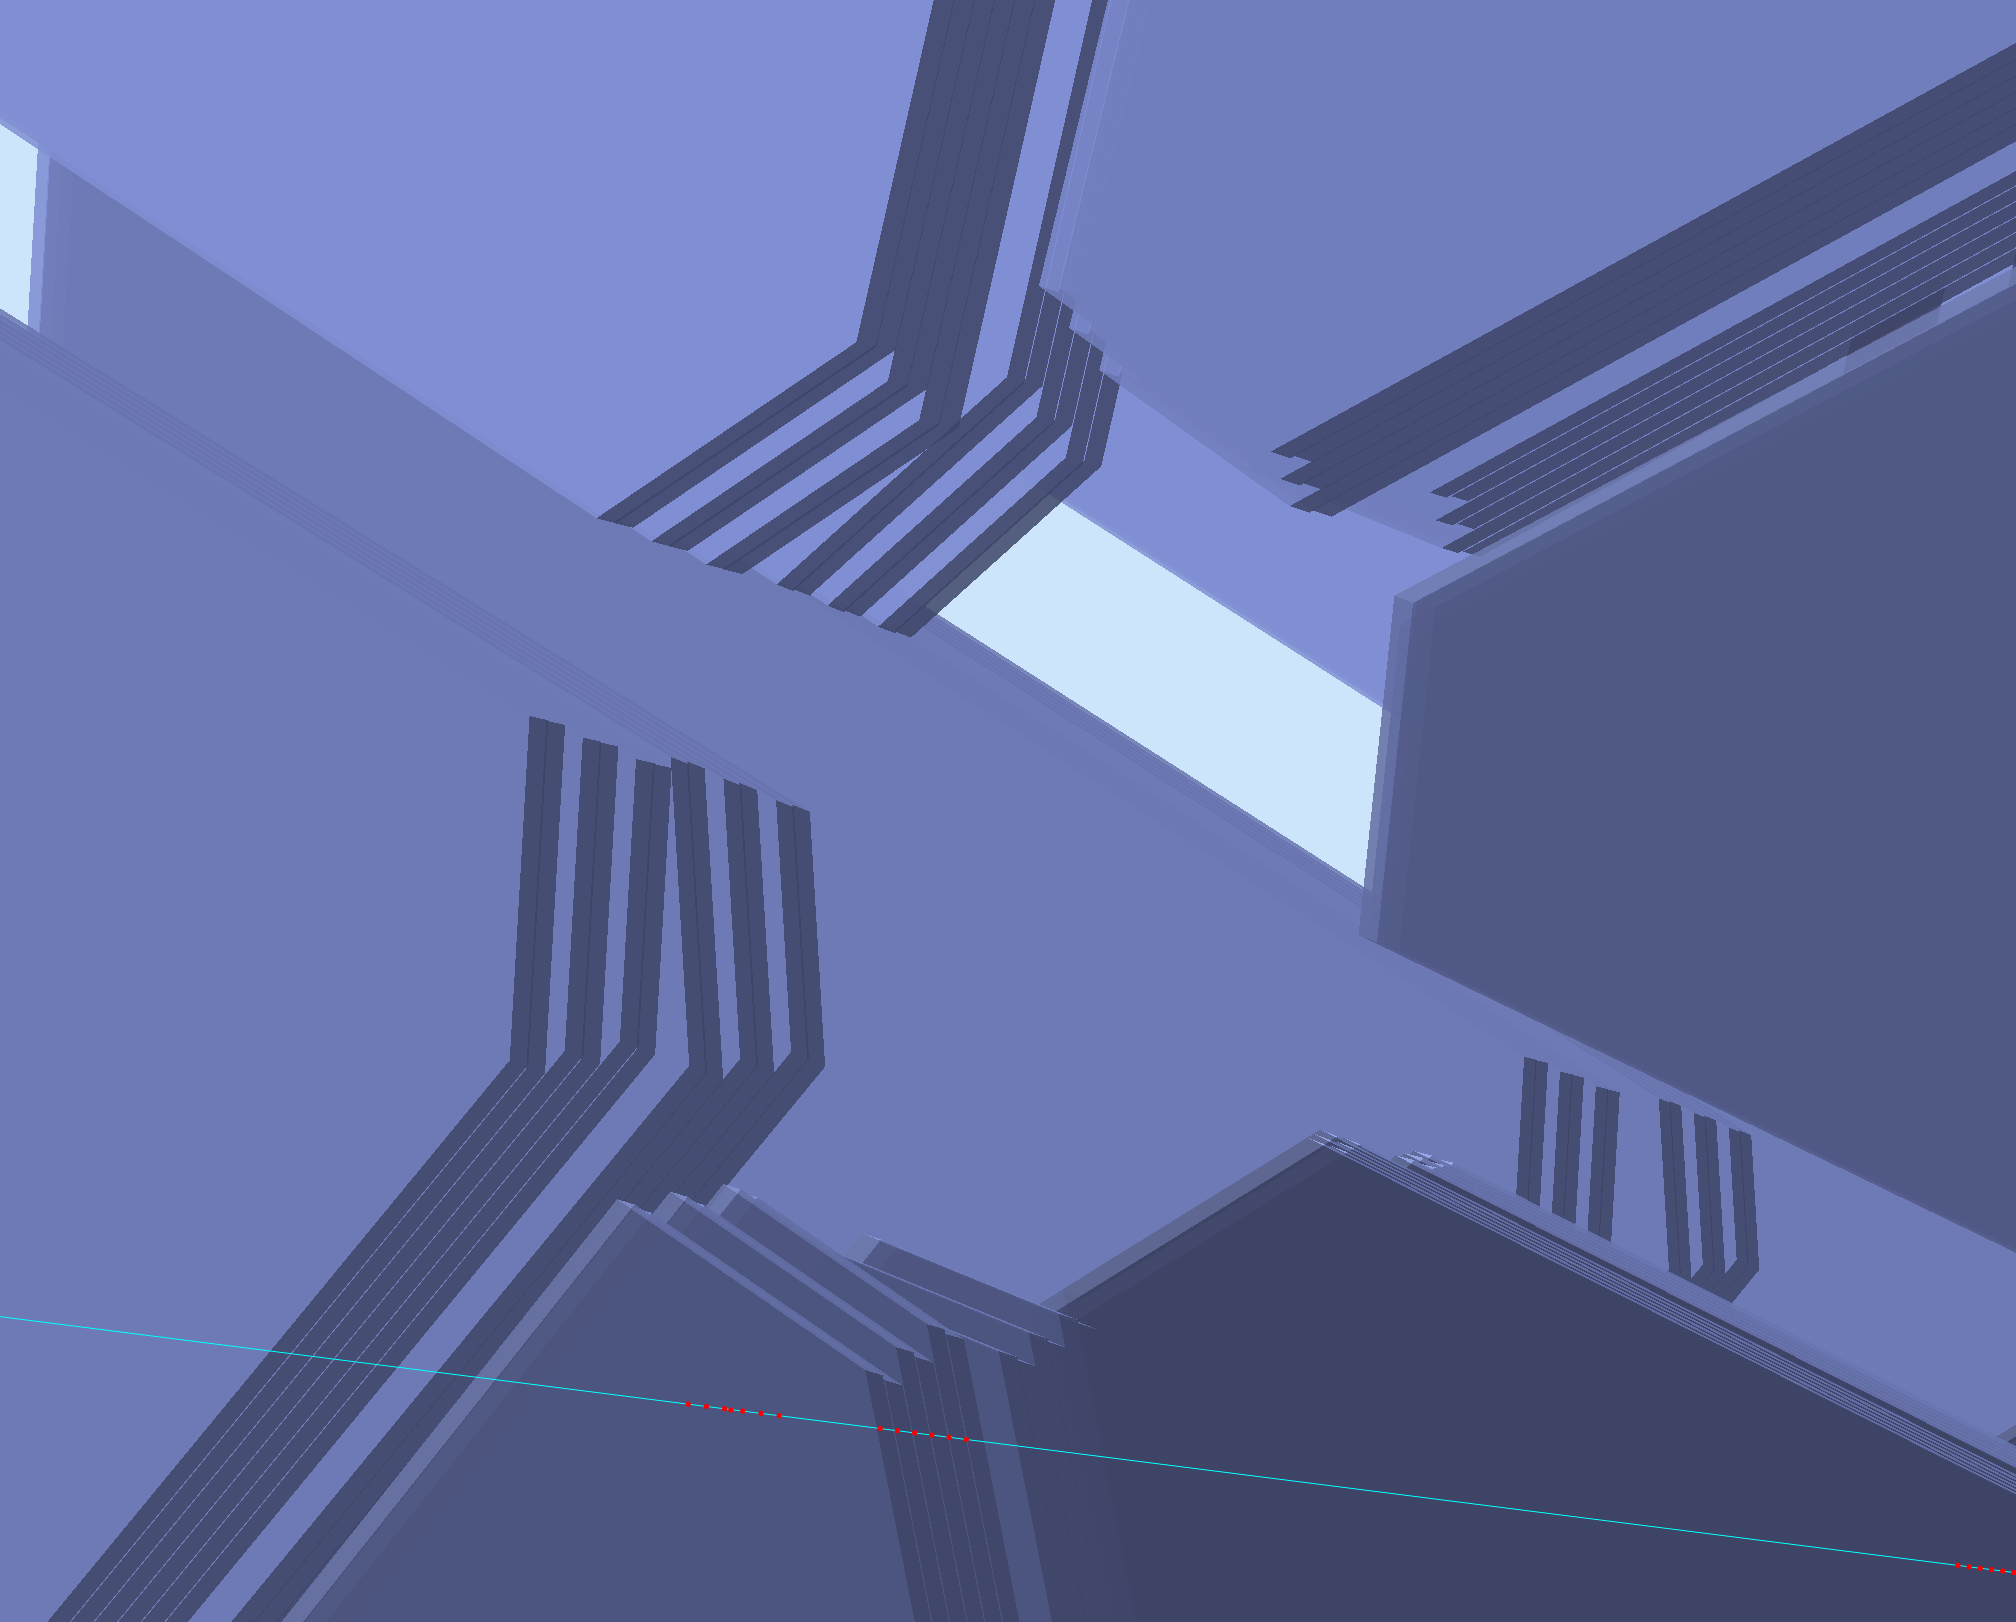
\includegraphics[width=0.95\columnwidth,keepaspectratio]{img/dcDetail.png}
	\caption{Top: the GEMC implementation of the FTOF geometry. The paddles are G4Boxes, embedded in trapezoid representing the mother volumes of each panel.
            Bottom: a zoom-in of the implementation shows the details of the individual paddles for Panel 1B (green) and Panel 1A (purple) }
	\label{fig:dcGeometry}
\end{figure}


\subsubsection{Geometry Git Location}

\subsection{Process ID}

\subsection{Digitization}



\subsubsection{ADC}
\subsubsection{TDC}

\subsubsection{Summary of CCDB Table used}

\subsection{Digitized Bank}

\subsubsection{Time Window}

\subsubsection{Process Routine Git Repository Location}


The DC hit process routine location in git is \url{https://github.com/gemc/source/blob/master/hitprocess/clas12/dc_hitprocess.cc}
